\documentclass{exam} % {{{1
\usepackage{amsmath, amssymb, amsthm, enumitem, float, caption, mathtools, tikz}
\usetikzlibrary{arrows, calc, decorations.markings, matrix, positioning}
\usepackage[titlenumbered, ruled]{algorithm2e}
\tikzset{>=latex}
\usepackage[final]{hyperref}

% mathbb and mathcal symbols
\newcommand{\NN}{\mathbb{N}}
\newcommand{\ZZ}{\mathbb{Z}}
\newcommand{\QQ}{\mathbb{Q}}
\newcommand{\RR}{\mathbb{R}}
\newcommand{\V}{\mathcal{V}}
\newcommand{\A}{\mathbb{A}}
\newcommand{\m}[1]{\mathbb{#1}}    % for models
\newcommand{\cl}[1]{\mathcal{#1}}  % for classes

% theorems and similar environments
\theoremstyle{plain}
  \newtheorem{thm}{Theorem}[section]  \newtheorem*{thm*}{Theorem}
  \newtheorem{claim}[thm]{Claim}      \newtheorem*{claim*}{Claim}
  \newtheorem{conj}[thm]{Conjecture}  \newtheorem*{conj*}{Conjecture}
  \newtheorem{cor}[thm]{Corollary}    \newtheorem*{cor*}{Corollary}
  \newtheorem{lem}[thm]{Lemma}        \newtheorem*{lem*}{Lemma}
  \newtheorem{prop}[thm]{Proposition} \newtheorem*{prop*}{Proposition}
\theoremstyle{definition}
  \newtheorem{defn}[thm]{Definition} \newtheorem*{defn*}{Definition}
  \newtheorem{ex}[thm]{Example}      \newtheorem*{ex*}{Example}
\theoremstyle{remark}
  \newtheorem{rk}[thm]{Remark}  \newtheorem*{rk*}{Remark}
\renewcommand{\Case}[1]{\smallskip \textbf{Case #1:}}
\newenvironment{claimproof} {
  \begin{proof}[Proof of claim]
  \renewcommand{\qedsymbol}{\ensuremath{\circ}}
  } {
  \end{proof}
  }

% custom commands
\DeclareMathOperator{\Cg}{Cg}
\DeclareMathOperator{\Clo}{Clo}
\DeclareMathOperator{\Con}{Con}
\DeclareMathOperator{\Rel}{Rel}
\DeclareMathOperator{\Sg}{Sg}
\DeclareMathOperator{\diag}{diag}
\newcommand{\bmat}[1]{ \begin{bmatrix} #1 \end{bmatrix} }
\newcommand{\Bmat}[1]{ \begin{Bmatrix} #1 \end{Bmatrix} }
\newcommand{\pmat}[1]{ \begin{pmatrix} #1 \end{pmatrix} }
\newcommand{\mat}[1]{ \begin{matrix} #1 \end{matrix} }
\newcommand{\vect}[1]{ \left< #1 \right> }
\newcommand{\ds}[1]{ \displaystyle{#1} }
\newcommand{\stack}[2]{\genfrac{}{}{0pt}{}{#1}{#2}}

% misc
\pagestyle{foot} \cfoot{\thepage}  % page numbering
\numberwithin{equation}{section}  % number equations within sections
\renewcommand{\d}{\;d}
\renewcommand{\epsilon}{\varepsilon}
\renewcommand{\phi}{\varphi}
\newcommand{\TODO}[1]{\noindent\textbf{TODO: #1}}

% exam documentclass settings
% restyle parts and subparts
\renewcommand{\thepartno}{\roman{partno}}
\renewcommand{\thesubpart}{\alph{subpart}}
\renewcommand{\subpartlabel}{(\thesubpart)}
\renewcommand{\subsubpartlabel}{(\thesubsubpart)}
% restyle multiple choice options
\renewcommand{\choicelabel}{\thechoice)}
% true or false questions (use \TFQuestion)
\newcommand{\TrueFalse}{\hspace*{0.25em}\textbf{True}\hspace*{1.25em}\textbf{False}\hspace*{1em}}
\newlength{\mylena} \newlength{\mylenb} \settowidth{\mylena}{\TrueFalse}
\newcommand{\TFQuestion}[1]{
  \setlength{\mylenb}{\linewidth} 
  \addtolength{\mylenb}{-121.15pt}
  \parbox[t]{\mylena}{\TrueFalse}\parbox[t]{\mylenb}{#1}
}

% document specific stuff
\renewcommand{\O}{\mathcal{O}}
\renewcommand{\P}{\texttt{P}}
\newcommand{\NP}{\texttt{NP}}
\newcommand{\CC}{\mathbb{C}}
\newcommand{\B}{\mathcal{B}}
\newcommand{\bra}[1]{ \left< #1 \right| }
\newcommand{\ket}[1]{ \left| #1 \right> }
\newcommand{\bracket}[2]{ \left< #1 \mid #2 \right> }
\tikzset{gate-c/.style = {draw, circle, inner sep=0.25em}}
\tikzset{gate-r/.style = {draw, rounded corners, rectangle}}
\tikzset{control/.style = {draw, fill, circle, inner sep=0.1em}}
%----------------------------------------------------------------------------}}}1
% Personal Stuff
\newcommand{\per}{\text{\textbf{per}}}
\DeclareMathOperator*{\Motimes}{\text{\raisebox{0.25ex}{\scalebox{0.8}{$\bigotimes$}}}}
\newcommand{\bigslant}[2]{{\raisebox{.2em}{$#1$}\left/\raisebox{-.2em}{$#2$}\right.}}

\begin{document}  
\printanswers
\title{Quantum Algorithms \\ Exam 2 Solutions}
\author{Patrick Canny}
\date{\today}
\maketitle
\vspace{-0.7em} \begin{center} \sc
  Due: 2019-05-15
\end{center} \vspace{2em}
\section{Introduction}

The goal of this paper is to give a careful specification of Shor's Algorithm. 
I will give a brief introduction to the algorithm's procedure (tersely noting
its major components and their basic functions), discuss the underlying theorems
that build the backbone of the algorithm's classical components, give careful
descriptions of the quantum components and how they work and finally provide 
an additional proof of correctness of the algorithm as a contained system.\\

Please note that throughout the paper, I will sometimes underline particular
expressions, i.e.
\[
  \ket{\underline{a^k}}
\]
This notation denotes that what is being referred to is ``the binary
representation of $a^k$'', rather than $a^k$ itself.\\

Without further ado, let's take a moment to examine the algorithm at a high level.
\section{The Algorithm}

At its core Shor's algorithm seeks to efficiently factor numbers. This makes it
an intriguing solution to breaking common cryptography schemes such as RSA 
encryption, which rely heavily on the computational complexity required to
factor a large number. Specifically, given some input $y$, Shor's algorithm 
will output $d, d \mid y$ with $Prob \geq 1 - \frac{1}{2^{k-1}}$ where $k$
is the number of prime divisors for $y$(see the "Classical Components" section
for more details on why this is the probability for success).\\

The terse specification of the algorithm is as follows:\\
\begin{center}
  \vspace*{1cm}
  \textit{(over)}
\end{center}
\begin{algorithm}[H]
  \SetAlgoLined
  \SetKwInOut{Input}{Input}
  \SetKwInOut{Output}{Output}
  \Input{$y > 1$}
  \Output{$d$ where $d\mid y$}
  \caption{Shor's Factoring Algorithm, tersely specified}
  \begin{enumerate}
    \item Check if $y$ is even ($y \mod 2 = 0$). If it is, output ``$d=2$''.
    \item Calculate the $k$th roots of unity for $k \in \{ 2, 3, \hdots \lfloor
      \log(y)\rfloor$. If $y = b^k$ for $b \in \m{Z}$ output ``$d = b$'' and exit
    \item Choose uniform $a \in \{2\hdots y-1\}$ and compute $b = \gcd(a, y)$.
      If $b > 1$, output ``$b = d$'' and exit.
    \item Compute $r = \per_y(a)$ using a Quantum circuit. If $r$ is odd, 
      then output ``$y$ is prime'' and exit.
    \item Compute $b = \gcd(a^{r/2}-1, y)$. Output ``$b = d$'' if $b > 1$ and 
      exit. 
    \item Output ``$y$ is prime'' and exit.
  \end{enumerate}
\end{algorithm}

As an overview, parts $1-3$ and $5$ of the above algorithm leverage 
classical components, while step $4$ is the quantum section.\\

It is important to describe the concept of $\per_y(a)$ in this problem. $\per_y
(a)$ denotes the ``period of $a$ with respect to $y$''. More specifically, say
we have some periodic function $f: \{0\hdots m\} \mapsto \{0\hdots m\}$. This
function being ``periodic'' means that $\forall x\in \{0\hdots m-t\}$ there is
$f(x) = f(x+t)$, but the values of $f(x), f(x+1), \hdots f(x+(r-1))$ are all
distinct.\\

Take $f(x) = a^x$.
\begin{align*}
  f(x) = f(z) 
  & \Leftrightarrow a^x = a^z\\
  & \Leftrightarrow a^{x-z} = 1\\
  & \Leftrightarrow x - z = k * \per_y(a)\\
  & \Leftrightarrow x - z \in \{k * \per_y(a) \mod(y) | k\in \m{Z}\}\\
\end{align*}
which equates period-finding to finding a hidden subgroup of 
$\bigslant{\m{Z}}{y \m{Z}}$.\\

This algorithm has polynomial runtime in the size of the log of the input. Specifically, its complexity is in 
\[
  \O((n^2)(\log^2(N))(\log^3(N)))
\]
where $n$ is the number of bits in the input, and $N = 2^n$.\\

Note that depending on the size of the input, the quantum circuit will need
to be adjusted slightly, as the number of input qubits indicates the size of
the input number.\\
\section{Classical Components}

Shor's algorithm utilizes a variety of classical approaches before even entering
a quantum component. The reason behind this is to attempt to find a divisor quickly without even needing the quantum portion of the circuit. In practice, 
these components may be rarely used, as in classic encryption algorithms large 
prime numbers are used. Additionally, the classical component serves to reduce
the problem of finding a divisor to the problem of finding the period, as 
described above.\\

As specified by the algorithm's procedure above, it is important to have a 
way to quickly compute the greatest common divisor(GCD) of two numbers. It is 
known that the Euclidian Algorithm's complexity is roughly  $\O(n^2)$, so
computing the GCD of a given pair of numbers can be done by a classical computer
efficiently.\\

It is also important to note that Shor's Algorithm's success hinges on a result
from number theory:
\begin{align*}
  a^t \equiv 1 \mod y
  &\Leftrightarrow a^t -1 \equiv 0 \mod y\\ 
  &\Leftrightarrow (a^{t/2} + 1)(a^{t/2} - 1) \equiv 0 \mod y\\ 
  &\Leftrightarrow  (a^{t/2}+1)(a^{t/2}-1) = k * y \text{ for some k }\\
\end{align*}
The interesting thing about this result is that it implies that a nontrivial 
divisor of $y$ can be found if $t$ is known in this equation. This is why it
is advantageous to design a quantum circuit which is able to efficiently compute
the period of $ax\mod y$. Note that this procedure will fail to find a 
nontrivial divisor of $y$ if $t$ is odd or if $x^{t/2} \equiv -1 \mod y$.\\

From here, it is possible to show that the procedure will produce a factor of 
$y$ with probability $\geq \frac{1}{2^{k-1}}$ where $k$ is the number of prime
divisors of $y$. Shor outlines a proof of this fact in his original paper
describing this algorithm, which I will paraphrase here:\\
\begin{proof}
  Take $y = \prod_{i=1}^{k} p_{i}^{\alpha_i}$, that is to say that it 
  is a product of $k$-many unique primes. Take $a_i = a\mod p_i^{\alpha_i}$ \\

  Let $r_i$ be $\per_{p_i^{\alpha_i}}(a_i)$, then $r$ is the least common
  multiple of all the $r_i$. If we consider the largest power of $2$ dividing
  each $r_i$, if all of these powers agree the algorithm will fail:
  \begin{itemize}
    \item if all the powers are $1$, then $r$ is odd and $r/2$ does not exist.
    \item if they are all equal and larger than $1$, then $x^{r/2} \equiv -1
      \mod y$ since $x^{r/2} \equiv -1 \mod p_i^{a_i}$ for all $i$. 
  \end{itemize}
  By the
  Chinese Remainder Theorem, choosing an $x\mod y$ at random is the same
  as choosing $i$ where $p_i^{a_i}$ is the $i$th prime power factor of $n$.
  This leads to the fact that, since the multiplicative group 
  ($\mod y^{\alpha}$) is cyclic for any odd prime power $y^{\alpha}$, each 
  of the previously attained powers of $2$ has at most a $50\%$ probability 
  of agreeing with any previous power, so when all $k$ of the powers are 
  considered, the total probability is at most $\frac{1}{2^{k-1}}$, so there
  is at least a $\frac{1}{2^{k-1}}$ chance that the selected value for $x$ is
  ``good'' and yields a factor for $y$ with this probability. 
\end{proof}

Finally, it is important to consider the probability of calculating the true
value of the period given a number of consecutive runs of this period finding
algorithm. Note that the quantum period finding procedure returns some 
value in the form $e^{2\pi i * k/t}$ where $t$ is the period. From here,
it is possible to extract the values for $k/t$, but we suppose that this
is represented as an irreducible fraction $\frac{k'}{t'}$. After running 
the algorithm $n$ times, we will have $\frac{k_1'}{t_1'},\frac{k_2'}{t_2'}
\hdots \frac{k_n'}{t_n'}$. Consider Lemma 13.2 from the textbook:\\
\begin{lem}
  If $n \geq 2$ fractions are obtained, then the probability that their 
  least common denominator is different from $t$ is less than $3*2^{-l}$
\end{lem}

Due to this lemma, the more times the quantum period-finding circuit is 
utilized, the more likely the period is to be correctly determined. Of course,
there is always a chance that this procedure could fail, but if there is a 
specified margin of error the algorithm can be run enough times in order to 
be within this error bound. 
\section{Quantum Components}

Now that we've shown that if it is possible to efficiently estimate the
period of $ax\mod y$, it is possible to effectively factor $y$, it is
time to describe the quantum components of Shor's algorithm.\\

The quantum components of the algorithm are as follows:
\begin{enumerate}
  \item A polynomial-size circuit to compute $\per_y(a)$ for $f = ax \mod y$ 
    with low error probability
  \item The inverse Quantum Fourier Transform, which is utilized by the 
    period finding algorithm.
\end{enumerate}

So, both of these components will be examined independently, though 
their results will be consequential in the result of the algorithm
as a whole. 
\begin{enumerate}
  \item 
    \textbf{Period Finding}\\
    The quantum circuit for period finding is given as follows:
  \begin{center} 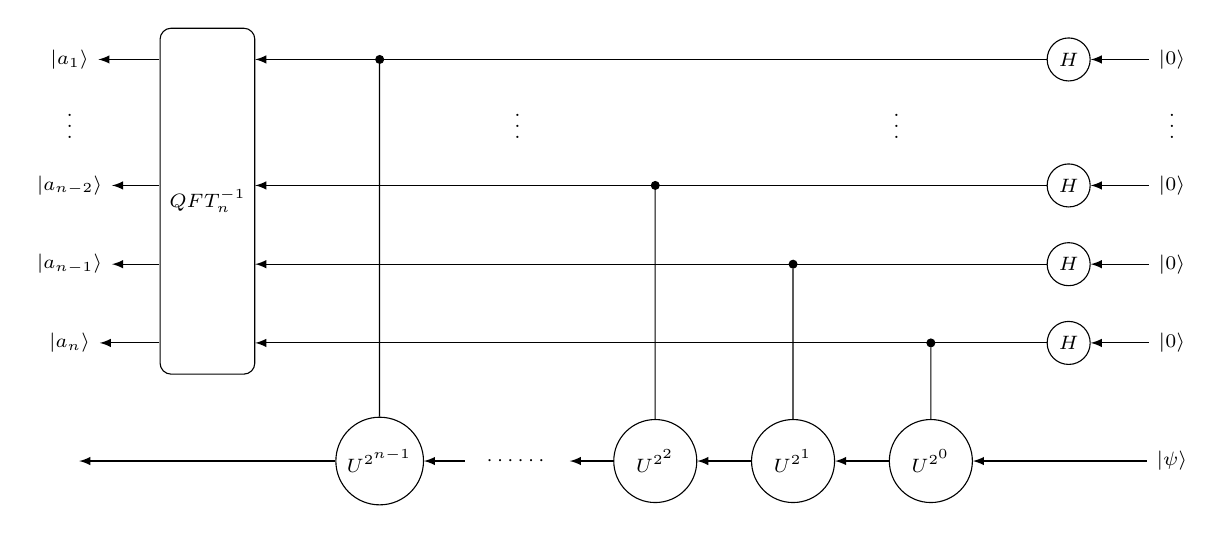
\begin{tikzpicture}[font=\scriptsize, xscale=1.75]
  \tikzset{Usize/.style = {minimum size=3em}}
  \path (0,0) node (r1) {$\ket{0}$}
      ++(-0.75,0) node[gate-c] (r1H) {$H$}
      ++(-5,0) node[control] (r1c) {}
      ++(-2.25,0) node (r1end) {$\ket{a_1}$}
        (r1)
      ++(0,-0.75) node {$\vdots$}
      ++(-2,0) node {$\vdots$}
      ++(-2.75,0) node {$\vdots$}
      ++(-3.25,0) node {$\vdots$}
        (r1)
      ++(0,-1.6) node (r2) {$\ket{0}$}
      ++(-0.75,0) node[gate-c] (r2H) {$H$}
      ++(-3,0) node[control] (r2c) {}
      ++(-4.25,0) node (r2end) {$\ket{a_{n-2}}$}
        (r2)
      ++(0,-1) node (r3) {$\ket{0}$}
      ++(-0.75,0) node[gate-c] (r3H) {$H$}
      ++(-2,0) node[control] (r3c) {}
      ++(-5.25,0) node (r3end) {$\ket{a_{n-1}}$}
        (r3)
      ++(0,-1) node (r4) {$\ket{0}$}
      ++(-0.75,0) node[gate-c] (r4H) {$H$}
      ++(-1,0) node[control] (r4c) {}
      ++(-6.25,0) node (r4end) {$\ket{a_n}$}
        (r4)
      ++(0,-1.5) node (rpsi) {$\ket{\psi}$}
      ++(-1.75,0) node[gate-c, Usize] (rpsiU0) {$U^{2^0}$}
      ++(-1,0) node[gate-c, Usize] (rpsiU1) {$U^{2^1}$}
      ++(-1,0) node[gate-c, Usize] (rpsiU2) {$U^{2^2}$}
      ++(-1,0) node (rpsidots)[minimum size=3.75em] {$\cdots\cdots$}
      ++(-1,0) node[gate-c, Usize] (rpsiUn) {$U^{2^{n-1}}$}
      ++(-2.25,0) node (rpsiend) {};
  \coordinate (t) at ($(r1)!0.5!(r4)$);
  \node[gate-r, minimum height=12.5em] at ($(t)+(-7,0)$) (Q) {$QFT_n^{-1}$};

  \foreach \i/\o in 
  {r1/r1H, r1H/Q.east|-r1end, Q.west|-r1end/r1end,
   r2/r2H, r2H/Q.east|-r2end, Q.west|-r2end/r2end,
   r3/r3H, r3H/Q.east|-r3end, Q.west|-r3end/r3end,
   r4/r4H, r4H/Q.east|-r4end, Q.west|-r4end/r4end,
   rpsi/rpsiU0, rpsiU0/rpsiU1, rpsiU1/rpsiU2, rpsiU2/rpsidots,
   rpsidots/rpsiUn, rpsiUn/rpsiend}
  {
    \draw[->] (\i) -- (\o);
  }
  \foreach \i/\o in {rpsiU0/r4c, rpsiU1/r3c, rpsiU2/r2c, rpsiUn/r1c}
  {
    \draw (\i) -- (\o);
  }
  \end{tikzpicture} \end{center} % }}}
    Where 
      \[
      U_a\ket{x} =  
      \begin{cases}
        &\ket{ax \mod y} \text{ if } 0\leq x < y-1\\
        &\ket{x}\text{ otherwise}
      \end{cases}
      \]
      raised to the various powers associated with it's position in the 
      circuit. \\

      At this point, it is important to talk about the state of this circuit
      at a variety of points in its execution:
      \begin{enumerate}
        \item The state directly after the initial application of all the $H$
          gates
        \item The state after all consecutive $U_a^{2^i}$ are applied
        \item The state after the application of $QFT_n^{-1}$ is applied,
          where the top $n$ qubits are measured. 
      \end{enumerate}
      so, each of these states will be considered independently.
      \begin{enumerate}
        \item The purpose of applying all the $H$ gates to the $n$ input
          qubits is to create a uniform distribution. We have
          \begin{align*}
            \big(H^{\otimes k} \otimes I\big)
            \big(\ket{0^n}\otimes\ket{\psi}\big)
            &=
            \big(H\ket{0}\big)^{\otimes n} \otimes \ket{\psi}\\
            &=
            \frac{1}{\sqrt{2}} (\ket{0} + \ket{1})^{\otimes n} 
            \otimes \ket{\psi}\\
            &=
            2^{-n/2} \sum_{x\in\{0,1\}^n} \ket{x} \otimes \ket{\psi}
          \end{align*}
          Recall that $k$ was previously selected in the classical portion of the
          algorithm. This state corresponds directly to the uniform 
          distribution we desire
          at this point, so now the continued applications of $U$ can be 
          discussed.\\
        \item
          First, let's call the application of all the $U_a^{2^i}$, 
          $\Upsilon(U)$.
          We will fix a $\ket{x} \in \{0,1\}^n$ and look at how the 
          aggregate operator $\Upsilon$ acts on it. Consider the following:
          \begin{align*}
            \Upsilon \big(\ket{x} \otimes \ket{\psi}\big)
            &= \ket{x} \otimes \Upsilon \ket{\psi}\\
            &= \ket{x} \otimes U_a^{\sum_{i=0}^{n-1} x_i*2^i}\ket{\psi}\\
            &= \ket{x} \otimes U^{\underline{x}}\ket{\psi}\qquad 
            \text{where }\underline{x}\text{ is the binary representation
            of the previously selected } x\\
            &= \ket{x} \otimes e^{2\pi i(x.\theta)}\ket{\psi}
          \end{align*}
          Where $\theta$ has the form $\frac{m}{t}$ and $t$ is the period
          described above. The reason this last part can be done is because
          $\psi$ is an eigenvector of $U_a$, which can be shown by the following
          calculations.
          \begin{align*}
            \ket{\xi} 
            &= \frac{1}{\sqrt{t}}\sum_{k=0}^{t-1} 
               e^{-2\pi i k/t}\ket{\underline{a^k}}\\
            &\implies 
            U_a\ket{\xi} = \frac{1}{\sqrt{t}}\sum_{k=0}^{t-1} 
            e^{-2\pi i k/t} U_a \ket{\underline{a^k}}\\
            &= \frac{1}{\sqrt{t}}\sum_{k=0}^{t-1} 
            e^{-2\pi i k/t}\ket{\underline{a^{k+1}}}\\
            &= \frac{1}{\sqrt{t}}\big(\ket{\underline{a}}+e^{-2\pi i 
            1/t}\ket{\underline{a^2}}+
            \hdots+e^{-2\pi i {t-1}/t}\ket{\underline{1}} \big)\\
            &= \frac{e^{-2\pi i({t-1}/t)}}{\sqrt{t}}\big(e^{-2\pi i 
            1/t}\ket{\underline{a}}+\hdots+\ket{\underline{1}} \big)\\
            &= e^{-2\pi i (t-1)/t}\ket{\xi}\\
            &= e^{2\pi i (1/t)}\ket{\xi}
          \end{align*}
          where $\ket{\underline{a^k}}$ denotes that $a^k$ is the binary 
          representation for the given choice of $a$ and $k$. The step where
          the power of $\ket{a^k}$ becomes $k+1$ is because of the definition
          of $U_a$: it will multiply a by itself, raising the power by $1$. So,
          we see that $U_a$ has eigenvectors of the form 
          \[
            \ket{\xi_k} = \frac{1}{\sqrt{t}}\sum_{m=0}^{t-1} e^{-2\pi i(k*m)/t}\\
          \]
          with corresponding eigenvalue
          \[
            \lambda_k = e^{2\pi i (k/t)}
          \]

          From here, it is possible to try and deduce the state of the circuit
          after the application of $\Upsilon(U)$:
          \[
            \Upsilon(U)\ket{\psi} 
            = 2^{{-n}/2}\sum_{x\in\{0,1\}^n} e^{2\pi i (\underline{x}\theta)}
            \ket{x}\otimes \ket{\psi}
          \]
          The information we wish to extract from this state is $\theta$ as it contains
          the phase information. This is why $QFT_n^{-1}$ is necessary in this 
          algorithm.
        \item Now that the state directly before entering the $QFT$ block 
          is known,
          we can now discuss the concrete application of the $QFT$. We will
          also discuss what the top $n$ qubits of the circuit represent
          after this application.
          The performance of this circuit will be discussed in the
          next section.\\
      \end{enumerate}
  \item
    \textbf{QFT}\\
    Note that in the actual implementation of the phase
    estimation circuit described above, the inverse Quantum Fourier Transform is 
    utilized. In this section, I will provide a description of a standard $QFT$,
    but note that since quantum computation is reversible that it is possible to get
    $QFT_n^{-1}$ by simply running this circuit backwards.\\

    Now, let's take a look at how the circuit is implemented, and show a few things
    about it's performance:\\
  \begin{center} 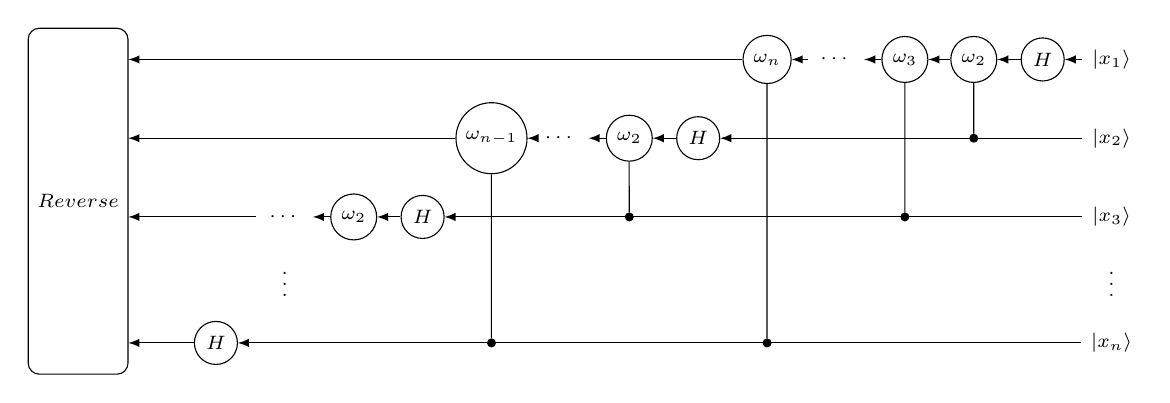
\begin{tikzpicture}[font=\scriptsize, xscale=1.75]
  \tikzset{Usize/.style = {minimum size=3em}}
  \path (0,0) node (r1) {$\ket{x_1}$}
      ++(-0.5,0) node[gate-c] (r1H) {$H$}
      ++(-0.5,0) node[gate-c] (r1o2) {$\omega_2$}
      ++(-0.5,0) node[gate-c] (r1o3) {$\omega_3$}
      ++(-0.5,0) node (r1dots)[minimum size=2em] {$\cdots$}
      ++(-0.5,0) node[gate-c] (r1on) {$\omega_{n}$}
      ++(-1,0) node (r1end) {}
        (r1)
      ++(0,-1) node (r2) {$\ket{x_2}$}
      ++(-1,0) node[control] (r2c1) {}
      ++(-2,0) node[gate-c] (r2H) {$H$}
      ++(-0.5,0) node[gate-c] (r2o2) {$\omega_2$}
      ++(-0.5,0) node (r2dots)[minimum size=2em] {$\cdots$}
      ++(-0.5,0) node[gate-c] (r2on1) {$\omega_{n-1}$}
      ++(-1,0) node (r2end) {}
        (r2)
      ++(0,-1) node (r3) {$\ket{x_3}$}
      ++(-1.5,0) node[control] (r3c1) {}
      ++(-2,0) node[control] (r3c2) {}
      ++(-1.5,0) node[gate-c] (r3H) {$H$}
      ++(-0.5,0) node[gate-c] (r3o2) {$\omega_2$}
      ++(-0.5,0) node (r3dots)[minimum size=2em] {$\cdots$}
      ++(-0.5,0) node (r3end) {}
        (r3)
      ++(0,-0.75) node {$\vdots$}
      ++(-6,0) node {$\vdots$}
        (r3)
      ++(0,-1.6) node (r4) {$\ket{x_n}$}
      ++(-2.5,0) node[control] (rnc) {}
      ++(-2,0) node[control] (rnc2) {}
      ++(-2,0) node[gate-c] (rnH) {$H$}
      ++(-1,0) node (r4end) {}
        (r4);
  \coordinate (t) at ($(r1)!0.5!(r4)$);
  \node[gate-r, minimum height=12.5em] at ($(t)+(-7.5,0)$) (Q) {$Reverse$};

  \foreach \i/\o in 
  {r1/r1H, r1H/r1o2, r1o2/r1o3, r1o3/r1dots, r1dots/r1on, r1on/Q.east|-r1end,
   r2/r2H, r2H/r2o2, r2o2/r2dots, r2dots/r2on1, r2on1/Q.east|-r2end,
   r3/r3H, r3H/r3o2, r3o2/r3dots, r3dots/Q.east|-r3end,
   r4/rnH, rnH/Q.east|-r4end}
  {
    \draw[->] (\i) -- (\o);
  }
  \foreach \i/\o in {r1o2/r2c1, r1o3/r3c1, r1on/rnc, r2o2/r3c2, r2on1/rnc2}
  {
    \draw (\i) -- (\o);
  }
  \end{tikzpicture} \end{center} % }}}
  
  Notable here is the fact that if an $\omega_k$ gate is shown to be directly on a rail,
  it really means that the given gate is really being partially controlled by that rail.
  The way this was denoted in class was to place the gates directly above the rail with
  two controls, but this has been omitted to save some space.\\

  Also note that this is a very general circuit, and that the patterns introduced here will 
  continue for all of the additional qubits in the sequence.\\

  The $QFT_n$ can be defined in the following way:
  \[
    \text{QFT}\ket{x} = 
    2^{-n/2} \Motimes_{l = 1}^{n} \big(\ket{0}+e^{2\pi i(x2^{-l})}\ket{1}\big)
  \]

  Additionally, $QFT_n^{-1}\ket{\gamma}$ can be defined to be
  \[
    2^{-n} \sum_x \sum_y 
    e^{2\pi i(y/2^n)(x-b)}
    e^{2\pi i(y\delta)}
    \ket{x}\ket{\psi}
  \]
  where $\delta$ is the error, and $0 \leq b \leq 2^{n-1}, b/2^n 
  = [0\hdots b_n]$\\ 

  The upshot to utilizing $QFT_n^{-1}$ is that it will be able to 
  extract the values for $\theta$ from the previous quantum circuit. This
  is because of the definition of $QFT_n^{-1}$:
  \[
    QFT_n^{-1}[1\hdots n]\ket{\gamma} = \ket{\theta_1\theta_2\hdots\theta_n}
  \]
  where $\ket{\gamma}$ is the state produced by the phase estimation circuit above, until 
  just before the quantum fourier transform. This is definitely a desirable state to achieve,
  since it is exactly what will allow the calculation of $t$ with precision noted in the
  classical components section.\\

  A given application of $H$ will have the following effect on a state:
  \begin{align*}
    H\ket{x_l} = 2^{-1/2}(\ket{0}+\epsilon_l\ket{1})
  \end{align*}
  where
  \begin{align*}
    \epsilon_l &= 
    \begin{cases}
      1 \text{ if  } x_l = 0\\
      -1 \text{ if } x_l = 1\\
    \end{cases}\\
    &=
    \begin{cases}
      e^{2\pi i} \text{ if  } x_l = 0\\
      e^{\pi i} \text{ if } x_l = 1\\
    \end{cases}\\
    &=
    \begin{cases}
      e^{2\pi i [0.0]} \text{ if  } x_l = 0\\
      e^{2\pi i[0.1]}\text{ if } x_l = 1\\
    \end{cases}\\
    &= e^{2\pi i[0.x_l]}
  \end{align*}
  
  The addition of the bracketed portions is to illustrate that additional bits of
  precision are being added with each $H$. The $[0.1], [0.0]$ are both base $2$ numbers,
  so $[0.1]$ behaves the same as $1/2$. This is what accounts for the addition of the 
  factor of $2$ on the first term. \\

  Just after the application of the first $\omega_2$ on the top rail, we can
  deduce the state and think about how consecutive applications of $\omega_k$ will
  result in a total transformation.\\
  \begin{align*}
    \ket{\gamma_1} 
    &= \Lambda(\omega_2) H\ket{x_1}\otimes\ket{x_2\hdots x_n}\\
    &= 2^{-1/2}\Lambda(\omega_2)\big((\ket{0}+e^{2\pi i[0.x_1]}\ket{1}) \otimes \\
    \ket{x_2\hdots x_n}\big)
    &= 2^{-1/2}\big((\ket{0}+e^{2\pi i[0.x_1x_2]}\ket{1}) \otimes 
    \ket{x_2\hdots x_n}\big)
  \end{align*}
  Where $\Lambda(\omega_2)$ is the controlled application of $\omega_2$ on the top rail.\\

  From here, the computation can be extended to $n$ applications of $\omega$, resulting in
  \[
    2^{-1/2}\big((\ket{0}+e^{2\pi i[0.x_1\hdots x_n]}\ket{1}) \otimes 
    \ket{x_2\hdots x_n}\big)
  \]
  This result will carry through the other rails, which will then be tensored with the 
  application of every other rail. Specifically, the pattern that emerges after the
  $\omega$ applications on the second rail is:
  \[
    2^{-1/2}\big((\ket{0}+e^{2\pi i[0.x_1\hdots x_n]}\ket{1}) \otimes 
    (\ket{0}+e^{2\pi i[0.x_2\hdots x_n]}\ket{1})\otimes\ket{x_3\hdots x_n} \big)
  \]
  After all applications, the final state of the circuit is
  \[
    2^{-n/2} 
    \Motimes_{l=1}^{n}
    \big(
    \ket{0} + e^{2 \pi i[0.x_{n-(l-1)}\hdots x_n]}\ket{1}
    \big) = QFT\ket{x}
  \]
  This shows that the $QFT$ performs as expected. Because the goal of this circuit in
  Shor's
  algorithm is to extract the bracketed portion of the expression, the circuit must be run
  in reverse to extract $\ket{x_1\hdots x_n}$.
\end{enumerate}
\section{Conclusions}
Shor's algorithm yields interesting and potentially highly consequential results.
The ability to factor numbers in polynomial time could be applied directly 
to cracking common cryptographic schemes. If quantum computation ever becomes
widely used, this would mean that some new form of cryptography would need to be
developed to ensure data security. We briefly discussed one such method in class:
The $k$-Local Hamiltonian. The potential issue with this problem is that it is
difficult to encode, especially when compared to RSA encryption. \\

It is important to note that the algorithm as described will find a divisor of a number
with high probability. If the total factorization of the number is desired, this
algorithm will need to be repeated on the result of dividing the input number by
the result of a previous run. Division can be done classically, and is efficient
enough to not make an impact on the runtime (I think it's $\O({n^2})$ in the
size of the input).\\
\end{document}
